% Options for packages loaded elsewhere
\PassOptionsToPackage{unicode}{hyperref}
\PassOptionsToPackage{hyphens}{url}
\PassOptionsToPackage{dvipsnames,svgnames*,x11names*}{xcolor}
%
\documentclass[
]{article}
\usepackage{lmodern}
\usepackage{amssymb,amsmath}
\usepackage{ifxetex,ifluatex}
\ifnum 0\ifxetex 1\fi\ifluatex 1\fi=0 % if pdftex
  \usepackage[T1]{fontenc}
  \usepackage[utf8]{inputenc}
  \usepackage{textcomp} % provide euro and other symbols
\else % if luatex or xetex
  \usepackage{unicode-math}
  \defaultfontfeatures{Scale=MatchLowercase}
  \defaultfontfeatures[\rmfamily]{Ligatures=TeX,Scale=1}
\fi
% Use upquote if available, for straight quotes in verbatim environments
\IfFileExists{upquote.sty}{\usepackage{upquote}}{}
\IfFileExists{microtype.sty}{% use microtype if available
  \usepackage[]{microtype}
  \UseMicrotypeSet[protrusion]{basicmath} % disable protrusion for tt fonts
}{}
\usepackage{xcolor}
\IfFileExists{xurl.sty}{\usepackage{xurl}}{} % add URL line breaks if available
\IfFileExists{bookmark.sty}{\usepackage{bookmark}}{\usepackage{hyperref}}
\hypersetup{
  colorlinks=true,
  linkcolor=blue,
  filecolor=Maroon,
  citecolor=Blue,
  urlcolor=Blue,
  pdfcreator={LaTeX via pandoc}}
\urlstyle{same} % disable monospaced font for URLs
\usepackage[margin=1in]{geometry}
\usepackage{graphicx}
\makeatletter
\def\maxwidth{\ifdim\Gin@nat@width>\linewidth\linewidth\else\Gin@nat@width\fi}
\def\maxheight{\ifdim\Gin@nat@height>\textheight\textheight\else\Gin@nat@height\fi}
\makeatother
% Scale images if necessary, so that they will not overflow the page
% margins by default, and it is still possible to overwrite the defaults
% using explicit options in \includegraphics[width, height, ...]{}
\setkeys{Gin}{width=\maxwidth,height=\maxheight,keepaspectratio}
% Set default figure placement to htbp
\makeatletter
\def\fps@figure{htbp}
\makeatother
\setlength{\emergencystretch}{3em} % prevent overfull lines
\providecommand{\tightlist}{%
  \setlength{\itemsep}{0pt}\setlength{\parskip}{0pt}}
\setcounter{secnumdepth}{-\maxdimen} % remove section numbering
\usepackage{fancyhdr}
\pagestyle{fancy}
\fancyhf{}
\rhead[\rightmark]{Ensayo II Geosistemas. 2nd Semester, 2021}
\lfoot[\thepage]{}
\rfoot[]{\thepage}
\newlength{\cslhangindent}
\setlength{\cslhangindent}{1.5em}
\newenvironment{cslreferences}%
  {\setlength{\parindent}{0pt}%
  \everypar{\setlength{\hangindent}{\cslhangindent}}\ignorespaces}%
  {\par}

\title{
\includegraphics[width=4cm,height=\textheight]{logoUMAG.jpg}}
\author{}
\date{\vspace{-2.5em}}

\begin{document}
\maketitle


\pagenumbering{gobble}

%\begin{titlepage}
\begin{flushleft}
\Large{\textbf{Ensayo II}}\\
\vspace*{2\baselineskip}
\begin{center}
\LARGE{\textbf{\textit{"El diablo está en los detalles";}}}\\
\LARGE{\textbf{Acidificación de los Océanos (OA) y dudas sobre el real impacto en las poblaciones marinas}}\\
\end{center}
\vspace*{3\baselineskip}
\Large{Curso GeoSistemas}\\
\vspace*{1\baselineskip}
\Large{2nd Semester 2021 }\\
\vspace*{3\baselineskip}
\end{flushleft}
\begin{flushright}
\large{\textbf{Mauricio Mardones Inostroza}}\\
\large{\textbf{Biólogo Marino}}\\
\vspace*{2\baselineskip}
\normalsize{PhD Student Antarctic and SubAntarctic Science Program}\\
\vspace*{1\baselineskip}
\normalsize{Universidad de Magallanes, Chile}\\
\vspace*{1\baselineskip}
\normalsize{\textbf{Profesor}}\\
Dr. Ricardo De Pol-Holz\\
\vspace*{1\baselineskip}
\normalsize{\textbf{}}\\
November, 2021
\end{flushright}

% \end{titlepage}


\hypersetup{linkcolor = black}
\newpage
\pagenumbering{roman}
%\tableofcontents
%\addcontentsline{toc}{section}{\contentsname}

\newpage



\pagenumbering{arabic}
\hypersetup{linkcolor = blue}

\fontsize{12}{26}
\selectfont{}

\hypertarget{introduccion}{%
\subsection{1. INTRODUCCION}\label{introduccion}}

\quad

Durante las últimas dos décadas, la disciplina de la oceanografía ha
sido testigo abuntante información respecto a la importancia de los
procesos químicos y su impacto en los distintos niveles de organización
biológica que existen en ecosistemas marinos, y a su vez, como estos
procesos han sido perturbados y acrecentados por la acción del hombre a
través de la emisión de gases de efecto invernadero en un contexto de
Cambio Clímatico (Cook et al., \protect\hyperlink{ref-Cook2013b}{2013}).
La Acidificación de los Océanos (AO) se ha convertido en un tópico que
ha despertado el interés de investigadores de todo el mundo (Figura 1) y
Chile no ha sido la excepción.

En términos prácticos, la AO implica una reducción del pH del agua de
mar (aumento concentración de iones de hidrógeno), actualmente causada
por un aumento dióxido de carbono (\({CO}_{2}\)) en la atmósfera.
Asociado Los cambios químicos incluyen una mayor concentración de iones
de bicarbonato y carbono inorgánico disuelto y una disminución
concentración de iones de carbonato en el océano (Williamson et al.,
\protect\hyperlink{ref-Williamson2021}{2021}). Aunque la química del
sistema de carbonato está bien documentada y comprendida, la
investigación sobre la biología e implicaciones ecológicas de la AO
antropogénica comenzó de forma potente y en serio hace unos 20 años
(Gattuso \& Hansson, \protect\hyperlink{ref-Gattuso2011}{2011}).

\begin{figure}

{\centering 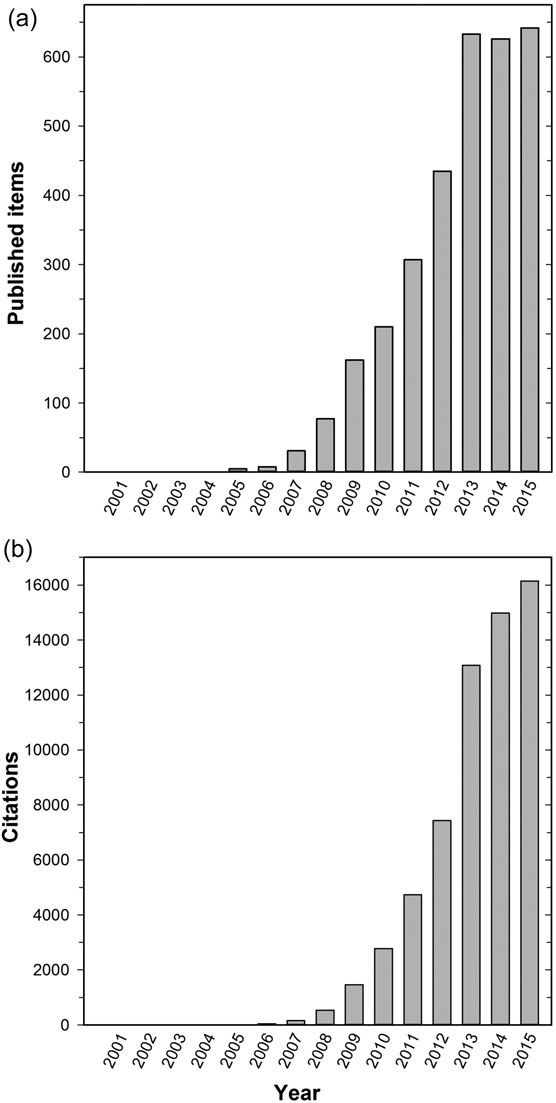
\includegraphics[width=0.6\linewidth]{images/Fig1} 

}

\caption{Crecimiento de citas y estudios relativos a la Acidificación de los Océanos en el mundo}\label{fig:unnamed-chunk-1}
\end{figure}

Esta investigación dice que una amplia gama de organismos marinos,
incluido el fitoplancton, invertebrados y peces, sintetizan alguna forma
de carbonato de calcio en sus estructuras. Las más llamativas de estas
estructuras son los esqueletos de corales, conchas de moluscos,
cocolitóforos y exoesqueletos de crustáceos. Varios estudios predicen
que la química del agua de mar no solo disminuirá formación de carbonato
de calcio (\({CaCO}_{3}^{-2}\)) en muchas organismos, sino también se
acelerará su disolución y/o erosión (Manríquez et al.,
\protect\hyperlink{ref-Manriquez2013}{2013}). Una amplia gama de
posibles consecuencias han sido identificados desde entonces, con
lucidez sobre la diversa vulnerabilidad de las especies de organismos
marinos.

En este sentido se han comprobado los efectos sobre los océanos,
ecosistemas y organismos de formar profusa. Sin embargo, y como toda
ciencia que madura en su transitar, durante el último tiempo este
\emph{``main topic''} ha tenido detractores que han objetado desde los
datos, métodos y experimentos que los han llevado a sus grandilocuentes
conclusiones. Este ensayo tiene como objetivo revisar parte de los
demostrados efectos del AO en las especies marinas, así como también las
legítimas dudas sobre la replicabilidad de los experimentos realizados,
los cuales han generado suspicacias en los últimos años. como objetivo
ulterior, se realizan reflexiones epistemologicas sobre la ciencia
misma, sus fortalezas y debilidades, las cuales pueden ser muy útiles en
el contexto de la AO.

\pagebreak

\hypertarget{cuerpo}{%
\subsection{2. CUERPO}\label{cuerpo}}

Respecto a las investigaciones acumuladas en los últimos años, existe en
Chile un cuerpo científico maduro que ha trabajado en esta línea con
profusos resultados en especies del medio marino. Todos estos trabajos
se han centrado en especies que generan estructuras calcareas
corporales, como copépodos y moluscos. Aguilera et al.
(\protect\hyperlink{ref-Aguilera2016}{2016}) encontraron que los cambios
en el pH producido por las descargas de los ríos pueden producir
respuestas en el fenótipo del copépodo nerítico \emph{Acartia tonsa}
frente a cambios en la química marina asociada a la AO. La variabilidad
adaptativa fue un factor determinante de las respuestas de los
copépodos. Este experimento permitió que estos copépodos toleraran una
mayor exposición a niveles altos de \(_PCO^2\), ya que sus tasas de
ingestión fueron en promedio 43\% superiores a las de los organismos
costeros. Sin embargo, uno de los mayores hallazgos fue identificar que
la adaptación a las fluctuaciones locales en el pH del agua de mar
desempeña un papel importante en la respuesta de las poblaciones
planctónicas a las condiciones asociadas a la AO.

Vargas et al. (\protect\hyperlink{ref-Vargas2017}{2017}) realizaron sus
análisis sobre distintos tipos de poblaciones marinas como copépodos,
mitílidos y gastrópodos. En ellos, encontraron que los factores de
estrés global, entre ellos, la la AO, constituyen un problema importante
y de rápida influencia para este tipo de organismos, asi como también su
en el funcionamiento de los servicios de ecosistémicos. Este análisis
fue realizado en el ecosistema costero del Sistema de la Corriente de
Humboldt (HCS) frente a Chile, el cual alberga un amplio gradiente
físico-químico latitudinal y temporal con considerable irregularidad en
las condiciones oceanográficas locales. Esta heterogeneidad puede, a su
vez, modular las tolerancias específicas de los organismos al estrés
climático en especies con poblaciones distribuidos a lo largo de este
gradiente ambiental. En el estudio observaron relaciones de respuesta
negativas en modelos de especies expuestos a cambios en la presión
parcial de \({CO}_{2}\) (\(_PCO^2\)). finalmente los autores proponen el
uso de un índice simple teniendo en cuenta la variabilidad natural de
\(_PCO^2\) a lo largo de los ecosistemas para una mejor interpretación
de las posibles consecuencias de la AO sobre las especies que habitan en
ecosistemas costeros variables.

Jahnsen-Guzmán et al. (\protect\hyperlink{ref-Jahnsen-Guzman2021}{2021})
probaron la capacidad de las especies para resistir variaciones de las
condiciones químicas del océano en un contexto de cambio. Estas
variaciones fueron consignadas en los sistemas estuarinos y la
estraficación vertical de la columna del agua, que puede crear
``refugios ambientales'' o distintas capas de agua con condiciones que
favorecen la aptitud de algunos individuos de la especie de chorito
chileno. La salinidad, el estado de saturación y los contenidos de
\({CO}_{3}\) en el agua de mar fueron algunos de los factores que mejor
explicaron las diferencias entre las dos capas. En tales condiciones
ambientales, las características de esta especie que respondieron a tal
variación fueron las tasas de crecimiento y calcificación, con valores
significativamente más altos a 4 m de profundidad, mientras que lo
contrario, el estrés metabólico aumentado, fue mayor en los choritos
criados y trasplantados a la superficie (1 m). Tales diferencias apoyan
la noción de un refugio ambiental, donde especies como los choritos
pueden encontrar mejores condiciones de crecimiento y lograr mayores
niveles de rendimiento. Estos resultados son relevantes considerando la
importancia de \emph{M. chilensis} como recurso para la acuicultura y
como especie formadora de hábitat. Además, estos resultados arrojan
luces sobre las respuestas variables exhibidas por los organismos
estuarinos a los cambios de pequeña escala en las características de la
columna de agua, lo que a su vez ayudará a comprender mejor las
respuestas de los organismos a los escenarios proyectados de cambio
climático global.

Yevenes et al. (\protect\hyperlink{ref-Yevenes2019}{2019}) investigaron
los efectos a mediano y largo plazo de la entrada de variables
biogeoquímicas en el Fiordo Reloncaví (41º40'S; 72º23'O) como resultado
de la erupción del volcán Calbuco. Este ecosistema soporta una mayores
producciones de cultivo de mitilidos de la patagonia Norte. Se testearon
los impactos de los cambios fisicoquímicos en la columna de agua sobre
los juveniles del chorito chileno \emph{Mytilus chilensis}. Después de
la erupción, un gran bloom de fitoplancton generó un aumento en pH, y
con ello un aumento de la acificación del estuario. Los resultados
sugieren un impacto localizado de la erupción volcánica en la superficie
del sistema de fiordos, y efectos a corto plazo en el sistema de
carbonatos y en las estructuras calcareas del chorito cultivado. Este
estudio contribuye a mejorar las estrategias de adaptación climática por
parte de la industria acuícola de choritos para enfrentar la AO y
cambios en las condiciones de escorrentía del sistema de fiordos en
donde estos se cultivan.

El loco \emph{Concholepas concholepas} es uno de los recursos económicos
y sociales mas importante de Chile. Manríquez et al.
(\protect\hyperlink{ref-Manriquez2013}{2013}) estudiaron como el OA
también puede influir en otros procesos biológicos clave, como la
supervivencia, el crecimiento y comportamiento de este tipo de
organismos. Estudiaron el impacto de la AO en la capacidad de recuperar
la posición despues del desalojo por motivo del oleaje. Este
comportamiento fue investigado bajo distintos niveles de \(_PCO^2\).
Estos resultados sugieren que la capacidad de volver a su posición en la
ontogenia temprana de \emph{C. concholepas} será afectada positivamente
por los niveles de \(_PCO^2\) esperados para finales del siglo XXI y
principios del próximo. Junto a la evaluación del impacto de la AO en
organismos, Vargas et al. (\protect\hyperlink{ref-Vargas2017}{2017}) y
Pérez et al. (\protect\hyperlink{ref-Perez2015}{2015}) estudiaron la
influencia de descargas de glaciares y ríos y como ello afecta a los
ciclos biogeoquímicos aportando carbono y nutrientes, y por ende
alterando la acidez de los sistemas.

De acuerdo con lo expuesto, es posible entender y comprobar el efecto de
la acidicifación del medio marino sobre organismos con estructuras
calcareas y su efectos. Sin embargo, algunos investigadores fueron
peligrosamente mas allá. Durante el inicio del siglo XXI, un grupo de
científicos liderados por Philip Munday (coautor de mas de 250 articulos
del tema\footnote{\url{https://researchonline.jcu.edu.au/view/jcu/B75BF971396A6653D2DCC47B11EB5981.html}})
abrieron un flanco relativo a los efectos de la cambiante química de los
océanos en los peces, afectando desde su fisiología, reproducción y
comportamiento. En unos de sus mas connotados trabajos (Munday et al.,
\protect\hyperlink{ref-Munday2013}{2013}) probaron el efecto de los
niveles de CO2 en un futuro cercano (490, 570, 700 y 960 de \(_PCO^2\))
(Figura 2) en las respuestas olfativas y niveles de actividad de
juveniles de trucha de coral, \emph{Plectropomus leopardus}, un pez de
arrecife piscívoro que también es una de las especies pesqueras más
importantes en la Gran Barrera de Arrecife Australiana. De acuerdo a
este experimeto en mesocosmo, el animal mostró un deterioro del
comportamiento si la \(_PCO^2\) se mantiene en niveles más altos, y
conllevaría impactos significativos en desempeño del juvenil de la
trucha, y por consiguiente, es probable que afecte la supervivencia y
sus presupuestos energéticos, con consecuencias incluso para las
interacciones predador-presa y pesquerías comerciales.

\begin{figure}

{\centering 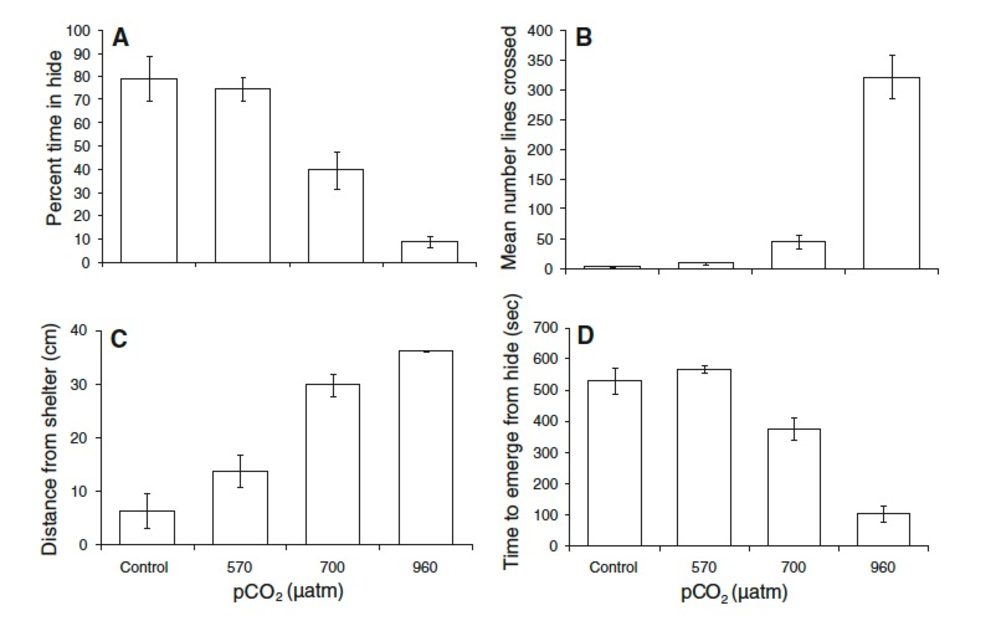
\includegraphics[width=1\linewidth]{images/Fig2} 

}

\caption{Comportamiento y niveles de actividad de trucha coralina despues de 28 días de exposición a distintos niveles de CO2 (Ex. Munday et al.2013}\label{fig:unnamed-chunk-2}
\end{figure}

En otro de los hallazgos del grupo liderado por Munday, (Miller et al.,
\protect\hyperlink{ref-Miller2013}{2013}) predicen que la acidificación
de los océanos tendrá un impacto negativo en la reproducción de muchas
especies marinas, ya sea al reducir el éxito de la fertilización o al
desviar la energía del esfuerzo reproductivo. En este estudio hicieron
los experimentos en estadios larvarios y juveniles del pez payaso
canela, \emph{Amphiprion melanopus}, de la Gran Barrera de Coral
Australiana. En este análisis, los autores proporcionan la primera
evidencia de los efectos potenciales de la acidificación del océano en
los atributos reproductivos claves de los peces marinos y demuestra un
efecto estimulante en respuesta al aumento de \(_PCO^2\).

Junto a estos experimentos, se presentaron cerca de un centenar mas de
la misma índole\footnote{\url{https://researchonline.jcu.edu.au/view/jcu/B75BF971396A6653D2DCC47B11EB5981.html}}
en un lapso de 15 años. El principal foco de investigaciòn del equipo
liderado por Munday, tenía como intención acumular evidencia del efecto
del aumento del nivel de \({CO}_{2}\) en el medio marino, demostrando
una serie de efectos sorprendentes en el comportamiento de los peces,
como hacerlos más audaces y dirigirlos hacia los productos químicos
producidos por sus depredadores. Este tipo de descubrimientos alcanzaron
fama mundial y fueron cubiertos por los mas prestigiosos medios
internacionales\footnote{\url{https://www.scientificamerican.com/article/ocean-acidification-can-m/}}.
Estas conclusiones llegaron incluso al informe de 2014 del Grupo
Intergubernamental de Expertos sobre el Cambio Climático (IPCC,
\protect\hyperlink{ref-IPCC2014}{2014}), advirtiendo los riesgos y las
``profundas consecuencias para la diversidad marina y las pesquerías
asociadas''.

Pero cuando la ciencia se avanza, crece y se acumula a pasos agigantados
y alcanza grandes estos niveles de notoriedad, ella también queda bajo
el escrutinio público con mayor fuerza y poder de fiscalización, como
fue el caso de este grupo y su foco de investigación. Analizando los
resultados del grupo de Munday, un grupo de investigadores liderados por
Clark et al. (\protect\hyperlink{ref-Clark2020}{2020}), trató de
replicar los experimentos anteriormente citados y no lograron reproducir
los resultados. Ellos establecieron que existían problemas importantes
considerados como \emph{``debilidades metodológicas o analíticas''} que
podrían haber llevado a resultados irreproducibles. Cabe señalar que el
grupo de Clark tiene un interés declarado por la ciencia desprolija y el
fraude científico. En el artículo, Clark et al.
(\protect\hyperlink{ref-Clark2020}{2020}) insinuaron incluso la
elaboración de malas conductas científicas. La prueba de replicabilidad
es una de las bases de la investigación moderna y es la forma en que la
comunidad se desafía a sí misma como un mecanismo para combatir la
subjetividad. La premisa de la replicabilidad es que la comunidad
científica puede corregir estos defectos.

Esta situación desencadenó largas disputas a la cual se sumaron otros
investigadores que fueron llamados a reevaluar los trabajos de Munday.
Estos identificaron los mismos problemas de reproducibilidad y
corroboraron lo descrito por Clark et al.
(\protect\hyperlink{ref-Clark2020}{2020}). Mas allá de esta disputa
científica, esto provocó un remezón en la investigación relativa a los
impactos de la AO en los ecosistemas marinos, estableciendo un manto de
duda sobre ella, generando con ello un escepticismo en la comunidad
científica internacional. Este tipo de controversias y revisión de los
procesos científicos tiene raíz en un aspecto mas profundo y filosófico
que se ha tratado de explicar mediante las bases conceptuales de la
epistemología.

Existe un fenomeno relacionado a la psicología humana y que está
ocurriendo en una amplia gama de campos científicos, desde la psicología
hasta la ecología, y podría ser descrito y conceptualizado con el nombre
de \emph{decline effect} o \emph{efecto de rechazo} (Lehrer,
\protect\hyperlink{ref-Lehrer2010}{2010}). Algunos efectos muy
comprobados comienzan a disminuir cuando se someten a repetición de sus
pruebas. Schooler (\protect\hyperlink{ref-Schooler2011a}{2011}) plantea
que muchos efectos descubiertos científicamente publicados en la
literatura parecen disminuir con el tiempo. Apodado el \emph{efecto de
rechazo}, esta desconcertante anomalía se descubrió por primera vez en
la década de 1930 en la investigación en parapsicología, en la que la
significación estadística de la supuesta evidencia de la capacidad
psíquica disminuyó a medida que se repetían los estudios (Schooler,
\protect\hyperlink{ref-Schooler2011a}{2011}).

Las explicaciones de este efecto incluyen la regresión a la media que
invisibiliza los detalles del cuerpo científico. Es más probable que se
informen resultados tempranos cuando los errores se combinan para
magnificar el efecto aparente, entonces los estudios publicados
mostrarán un sesgo sistemático hacia hallazgos inicialmente exagerados,
que posteriormente se autocorrigen estadísticamente. Otro aspecto mas
atingente con el asunto de este ensayo dice relación con el sesgo de
publicación. Esto señala que es posible que los investigadores solo
puedan publicar hallazgos iniciales sobre un efecto cuando es
especialmente grande y esperado que así ocurra, mientras que los
estudios que lo secudan y que presentan aspectos menos conspicuos
podrían ser capaces de reportar efectos más pequeños.

Por otro lado, muchos investigadores, como el grupo de Munday, trabajan
con un sesgo en el cual buscan encontrar qué resultados quieren, y eso
puede influir en los resultados e incurrir en errores y desproligidad al
momento de establecer sus experimentos. Esta situación a su vez
entorpece la replicabilidad de la ciencia. La acumulación de evidencia
científica para corroborar los hallazgos que están de moda o concitan
gran aceptación del a comunidad ha sido descrito con lucidez por Thomas
Khun como \emph{``ciencia normal''}. Sin embargo, la acumulación del
conocimiento en cualquier tòpico puede comenzar a parecer cada vez más
incierto, y con ripios, que fue lo que aconteció con los hallazgos
relativos al impacto del AO sobre el comportamiento de peces tropicales.

En este sentido, es posible comprender que la profusa evidencia que
había respecto a los efectos del AO sobre los ecosistemas marinos y que
se estaba acumulando durante las dos últimas décadas, ocultaron otros
estudios con resultados negativos. Por lo tanto, fue muy complejo
\emph{``nadar contra la corriente''} y publicar resultados que
promovieran cuestionamientos a la corriente principal. Sin embargo, y
como todo proceso de conocimiento científico, existen también, a veces
muy ocultas, pequeñas señales que pueden iluminar el camino desde otra
perspectiva y generar los cambios de paradigma, que son, a fin de
cuentas, los procesos cognitivos que perfeccionan el progreso del
conocimiento científico.

\pagebreak

\hypertarget{discusion}{%
\subsection{3. DISCUSION}\label{discusion}}

El cambio climático no es lineal en sus impactos, pero sus resultados
influyen en la ciclicidad normal de los patrones climáticos que afectan
a la naturaleza y a los ecosistemas allí contenidos. Uno de los mas
significativos impactos tiene relación con la Acidificación de los
Océanos. Este fenomeno de causas antropogénicas esta descrito como el
proceso en el cual el océano absorbe cantidades significativas de
\({CO}_{2}\) de la atmósfera. Las concentraciones de \({CO}_{2}\)
atmosférico siguen aumentando como resultado de las actividades humanas,
como el uso de combustibles fósiles y el cambio de uso de la tierra. En
este proceso el océano juega un papel fundamental en la desaceleración
de la tasa de cambio climático, absorbiendo alrededor del 30 \% de las
emisiones antropogénicas anuales (Le Quéré et al.,
\protect\hyperlink{ref-LeQuere2016}{2016}). a pesar de este rol
fundamental del océano, existe un desequilibrio previamente descrito
entre los gases en el aire y en el agua, por lo tanto, el valor del pH
del océano ha disminuido, es decir, el océano se acidifica cuando el
agua reacciona con el \({CO}_{2}\). Esto trae como consecuencia que el
agua ácida altera la capacidad de los organismos calcificados para para
desarrollar sus procesos fisiológicos y biológicos de manera regular.

Con este contexto, el presente ensayo tuvo dos objetivos definidos. El
primero dice relación con identificar y desplegar una serie de estudios
que comprueban el impacto del AO sobre organismos marinos que son
influidos directamente por los procesos quimicos derivados de los
niveles del \({CO}_{2}\) en el medio para formar las estructuras
corporales, como son copépodos, mitílidos y gastrópodos. En este
analisis no existe mayor cuestionaniento respecto a los hallazgos de los
distintos autores nacionales e internacionales. El segundo objetivo, se
desprende del primero, en donde se cuestiona la acumulación de
conocimiento que arrastra este tópico y el cuerpo cientifico que trabaja
en ello. En este aspecto, se cuestiona extender la ciencia asociada a la
AO y sus efectos en el comportamiento y reproducción de peces
tropicales. Este tipo de investigación acumuló profusa evidencia, pero
tambien ha sido parte del ojo fiscalizador de la comunidad científica, y
es ahí donde se identifican conductas no deseadas, las que tienen
implicancias directas en los resultados y grandilocuentes conclusiones
emanadas.

Aquí se podría desprender un problema de información selectiva, la cual
tiene sus raíces en un defecto cognitivo fundamental, que es que nos
gusta demostrar que estamos bien y evitamos estar equivocados, y lo que
es peor, no demostrar lo que nadie quiere escuchar. Estas conductas son
los pequeños detalles que socaban la confianza que existe en la
humanidad sobre el desarrollo de la ciencia. El \emph{efecto de rechazo}
es preocupante porque nos recuerda lo difícil que es probar algo y que a
su vez nos gusta fingir que nuestros experimentos definen la verdad para
nosotros.

Es por ello que, cada vez que un tema científico se vuelve importante y
congrega adeptos y loas corroborando lo que todos quieren escuchar, es a
veces necesario prestar atención a los detalles, dado que muchas veces
\emph{``el diablo está en los detalles''}\ldots{}

\pagebreak

\hypertarget{referencias}{%
\subsection*{4. REFERENCIAS}\label{referencias}}
\addcontentsline{toc}{subsection}{4. REFERENCIAS}

\hypertarget{refs}{}
\begin{cslreferences}
\leavevmode\hypertarget{ref-Aguilera2016}{}%
Aguilera, V. M., Vargas, C. A., Lardies, M. A., \& Poupin, M. J. (2016).
Adaptive variability to low-pH river discharges in Acartia tonsa and
stress responses to high PCO2 conditions. \emph{Marine Ecology},
\emph{37}(1), 215--226. \url{https://doi.org/10.1111/maec.12282}

\leavevmode\hypertarget{ref-Clark2020}{}%
Clark, T. D., Raby, G. D., Roche, D. G., Binning, S. A., Speers-Roesch,
B., Jutfelt, F., \& Sundin, J. (2020). Ocean acidification does not
impair the behaviour of coral reef fishes. \emph{Nature 2020 577:7790},
\emph{577}(7790), 370--375.
\url{https://doi.org/10.1038/s41586-019-1903-y}

\leavevmode\hypertarget{ref-Cook2013b}{}%
Cook, J., Nuccitelli, D., Green, S. A., Richardson, M., Winkler, B.,
Painting, R., Way, R., Jacobs, P., \& Skuce, A. (2013). Quantifying the
consensus on anthropogenic global warming in the scientific literature.
\emph{Environmental Research Letters}, \emph{8}(2).
\url{https://doi.org/10.1088/1748-9326/8/2/024024}

\leavevmode\hypertarget{ref-Gattuso2011}{}%
Gattuso, J. P., \& Hansson, L. (2011). \emph{Ocean Acidification} (p.
408).
\url{https://global.oup.com/academic/product/ocean-acidification-9780199591091?cc=us\%7B/\&\%7Dlang=en\%7B/\&\%7D\%7B/\#\%7D}

\leavevmode\hypertarget{ref-IPCC2014}{}%
IPCC. (2014). \emph{Climate Change 2014: Synthesis Report. Contribution}
(p. 169).

\leavevmode\hypertarget{ref-Jahnsen-Guzman2021}{}%
Jahnsen-Guzmán, N., Lagos, N. A., Lardies, M. A., Vargas, C. A.,
Fernández, C., San Martín, V. A., Saavedra, L., Cuevas, L. A., Quijón,
P. A., \& Duarte, C. (2021). Environmental refuges increase performance
of juvenile mussels Mytilus chilensis: Implications for mussel seedling
and farming strategies. \emph{Science of the Total Environment},
\emph{751}, 141723.
\url{https://doi.org/10.1016/j.scitotenv.2020.141723}

\leavevmode\hypertarget{ref-Lehrer2010}{}%
Lehrer, J. (2010). \emph{The Truth Wears Off}.
\url{https://www.newyorker.com/magazine/2010/12/13/the-truth-wears-off}

\leavevmode\hypertarget{ref-LeQuere2016}{}%
Le Quéré, C., Andrew, R. M., Canadell, J. G., Sitch, S., Ivar
Korsbakken, J., Peters, G. P., Manning, A. C., Boden, T. A., Tans, P.
P., Houghton, R. A., Keeling, R. F., Alin, S., Andrews, O. D., Anthoni,
P., Barbero, L., Bopp, L., Chevallier, F., Chini, L. P., Ciais, P.,
\ldots{} Zaehle, S. (2016). Global Carbon Budget 2016. \emph{Earth
System Science Data}, \emph{8}(2), 605--649.
\url{https://doi.org/10.5194/ESSD-8-605-2016}

\leavevmode\hypertarget{ref-Manriquez2013}{}%
Manríquez, P. H., Jara, M. E., Mardones, M. L., Navarro, J. M., Torres,
R., Lardies, M. A., Vargas, C. A., Duarte, C., Widdicombe, S.,
Salisbury, J., \& Lagos, N. A. (2013). Ocean Acidification Disrupts Prey
Responses to Predator Cues but Not Net Prey Shell Growth in Concholepas
concholepas (loco). \emph{PLOS ONE}, \emph{8}(7), e68643.
\url{https://doi.org/10.1371/JOURNAL.PONE.0068643}

\leavevmode\hypertarget{ref-Miller2013}{}%
Miller, G. M., Watson, S. A., Mccormick, M. I., \& Munday, P. L. (2013).
Increased CO2 stimulates reproduction in a coral reef fish. \emph{Global
Change Biology}, \emph{19}(10), 3037--3045.
\url{https://doi.org/10.1111/GCB.12259}

\leavevmode\hypertarget{ref-Munday2013}{}%
Munday, P. L., Pratchett, M. S., Dixson, D. L., Donelson, J. M., Endo,
G. G. K., Reynolds, A. D., \& Knuckey, R. (2013). Elevated CO2 affects
the behavior of an ecologically and economically important coral reef
fish. \emph{Marine Biology}, \emph{160}(8), 2137--2144.
\url{https://doi.org/10.1007/S00227-012-2111-6/FIGURES/2}

\leavevmode\hypertarget{ref-Perez2015}{}%
Pérez, C. A., DeGrandpre, M. D., Lagos, N. A., Saldías, G. S., Cascales,
E. K., \& Vargas, C. A. (2015). Influence of climate and land use in
carbon biogeochemistry in lower reaches of rivers in central southern
Chile: Implications for the carbonate system in river-influenced rocky
shore environments. \emph{Journal of Geophysical Research:
Biogeosciences}, \emph{120}(4), 673--692.
\url{https://doi.org/10.1002/2014JG002699}

\leavevmode\hypertarget{ref-Schooler2011a}{}%
Schooler, J. (2011). Unpublished results hide the decline effect.
\emph{Nature 2011 470:7335}, \emph{470}(7335), 437--437.
\url{https://doi.org/10.1038/470437a}

\leavevmode\hypertarget{ref-Vargas2017}{}%
Vargas, C. A., Lagos, N. A., Lardies, M. A., Duarte, C., Manríquez, P.
H., Aguilera, V. M., Broitman, B., Widdicombe, S., \& Dupont, S. (2017).
Species-specific responses to ocean acidification should account for
local adaptation and adaptive plasticity. \emph{Nature Ecology and
Evolution}, \emph{1}(4), 1--7.
\url{https://doi.org/10.1038/s41559-017-0084}

\leavevmode\hypertarget{ref-Williamson2021}{}%
Williamson, P., Portner, H. O., Widdicombe, S., \& Gattuso, J. P.
(2021). Ideas and perspectives: When ocean acidification experiments are
not the same, repeatability is not tested. \emph{Biogeosciences},
\emph{18}(5), 1787--1792. \url{https://doi.org/10.5194/bg-18-1787-2021}

\leavevmode\hypertarget{ref-Yevenes2019}{}%
Yevenes, M. A., Lagos, N. A., Farías, L., \& Vargas, C. A. (2019).
Greenhouse gases, nutrients and the carbonate system in the Reloncaví
Fjord (Northern Chilean Patagonia): Implications on aquaculture of the
mussel, Mytilus chilensis, during an episodic volcanic eruption.
\emph{Science of the Total Environment}, \emph{669}, 49--61.
\url{https://doi.org/10.1016/j.scitotenv.2019.03.037}
\end{cslreferences}

\end{document}
